\documentclass{beamer}
\usetheme{Copenhagen}
\usepackage{graphicx}
\usepackage{tikz}
% \usepackage[ruled,vlined,english]{algorithm2e}
% \renewcommand{\thealgocf}{}
% \usepackage{hyperref}
\usepackage{newunicodechar}
\newunicodechar{️}{}

\author[Digital twin in the Environment]{\large Hanna CHETOUANE, Narmimane ZAOUACHE \\ \vspace{-0.8cm} \date{\today}}
\title[Urban mocroclimate]{\textbf{Digital twin in the Environment:} \\ Urban microclimate}



\begin{document}

\begin{frame}
    \titlepage
    \vspace{-0.7cm}
    \begin{center}
        UFR of Mathematics and Informatics - University of Strasbourg 
        \\[0.6cm] 
        \textit{How do digital twins help us understand the effects of urban development on the microclimate?}
    \end{center}
\end{frame} 


\begin{frame}{Plan}
    % \tableofcontents    
    \begin{enumerate}
        \item Context
        \item What is a digital twin?
        \item How a digital twin works
        \item Methods
        \item Architecture and Pipeline
        \item Data \& Instrumentation — Data Budget (Urban Microclimate)
        \item V\&V \& UQ — Verification, Validation \& Uncertainty Quantification
        \item Transfer \& Deployment — CI/CD, Edge vs Cloud, Observability, Risks
        \item Perspectives
        \item Limitations
    \end{enumerate}
\end{frame}


\begin{frame}{Context}
    \small
    % \vspace{-1cm}
    % \begin{flushright}
    %     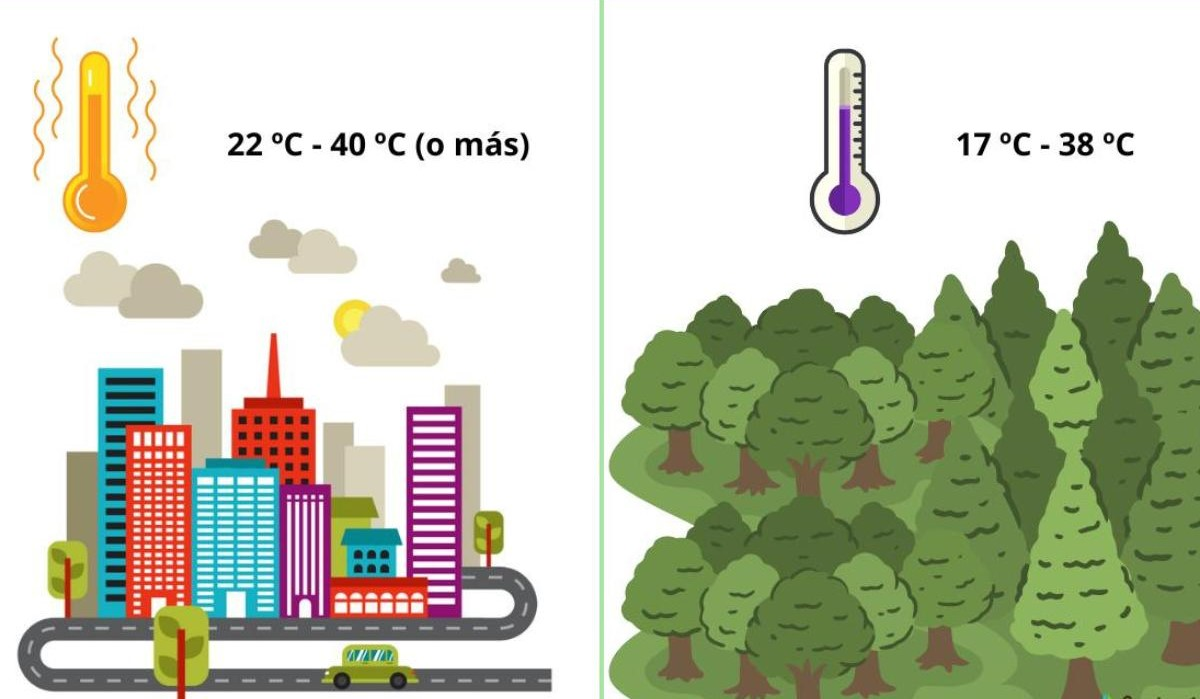
\includegraphics[width=0.4\textwidth]{images/ilot_de_chaleur.jpg}
    % \end{flushright}
    
    \begin{columns}[T]
    \begin{column}{0.6\textwidth}
    \begin{itemize}
        \setlength\itemindent{0.3cm}
        \item Ecology and climate have become major issues, especially in cities where heat islands are developing
        \item Solutions: Greening, choice of suitable materials, and redesigned urban planning
        \end{itemize}
    \end{column}

    \begin{column}{0.4\textwidth}
        \vspace{-0.3cm}
        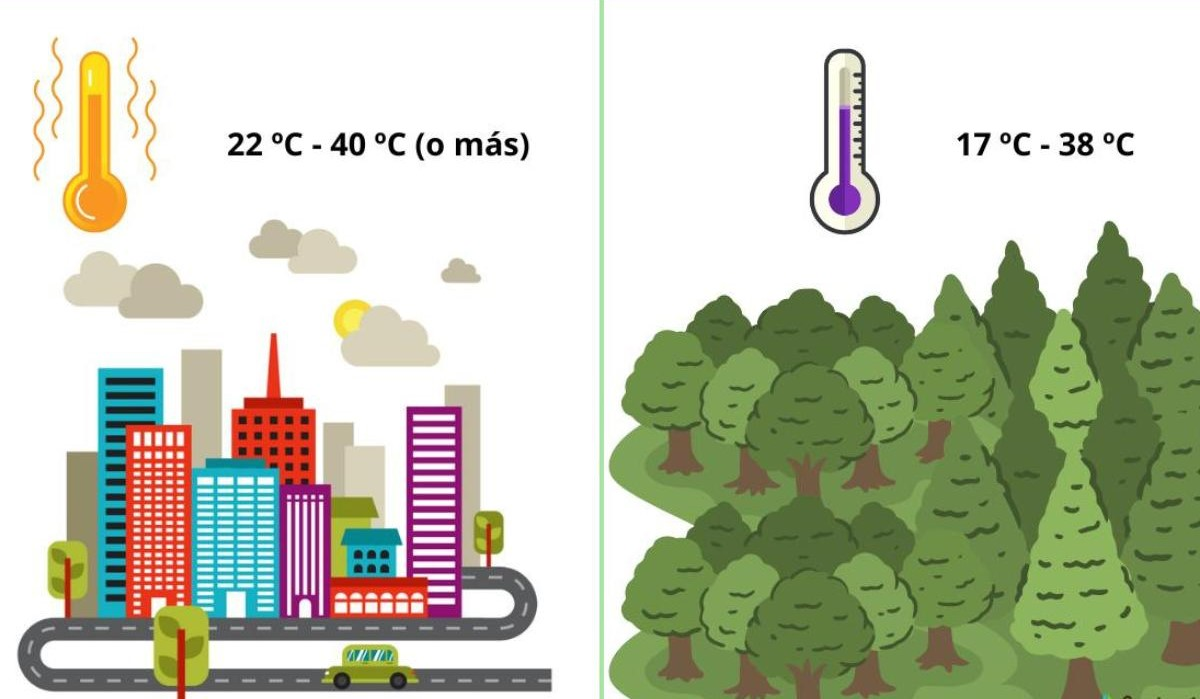
\includegraphics[width=1\textwidth]{images/ilot_de_chaleur.jpg}
    \end{column}
    \end{columns}

    \vspace{0.2cm}

    \begin{itemize}
        \item Local authorities must therefore make decisions on the development strategies to be adopted and evaluate their environmental and health impact.
    \end{itemize}
    $\rightarrow$ Simulate and predict the effects of these choices on the urban microclimate and public health $\Rightarrow $ \textbf{Digital twin}
\end{frame}


\begin{frame}{What is a digital twin?}
    \small
    \begin{itemize}
        \item Virtual and dynamic replica of a real system, which, when coupled with simulation tools, allows its behavior to be analyzed and predicted under different conditions
        \item Based on real data (meteorological and urban) from sensors, observations, or physical models
    \end{itemize}
    \begin{center}
        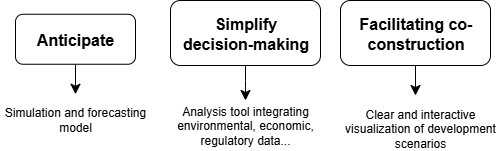
\includegraphics[width=0.7\textwidth]{images/objectifs_jm.png} \\
    \end{center}
    Current challenge in France: JNFT project led by IGN, Cerema, and Inria, which aims to create a multi-thematic digital twin covering the French territory
\end{frame}


\begin{frame}{How a digital twin works} %Architecture et pipeline}
    \hspace*{-0.5cm}
    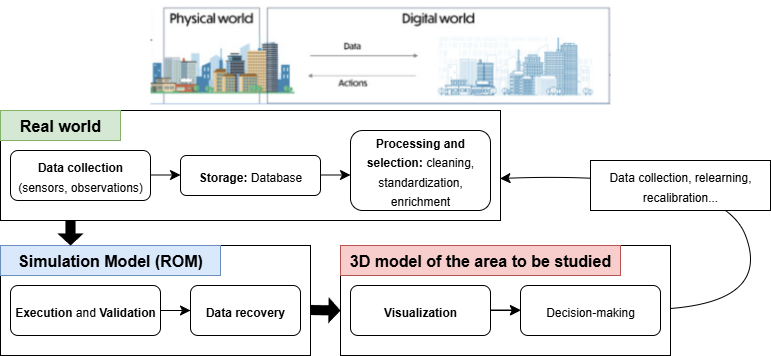
\includegraphics[width=1.1\textwidth]{images/pipeline.png} \\
\end{frame}


\begin{frame}{Methods}
    \small
    %Modélisation de phénomènes physiques
    % pour résoudre numériquement par FEM, VM, DM
    \begin{columns}[T]
        \begin{column}{0.45\textwidth}
            \textbf{Physical:} \\
            \begin{itemize}
                \item Data (weather, material properties, air composition)
                \item Microclimate
            \end{itemize}
        \end{column}
        \begin{column}{0.1\textwidth}
            \begin{center}
                \tikz[scale=1]{\draw[->, very thick] (0,0) -- (0.5,0);}
            \end{center}
        \end{column}
        \begin{column}{0.45\textwidth}
            \textbf{Digital:}
            \begin{itemize}
                \item Parameters
                \item 3D mesh model
            \end{itemize}
            \vspace{0.3cm}
            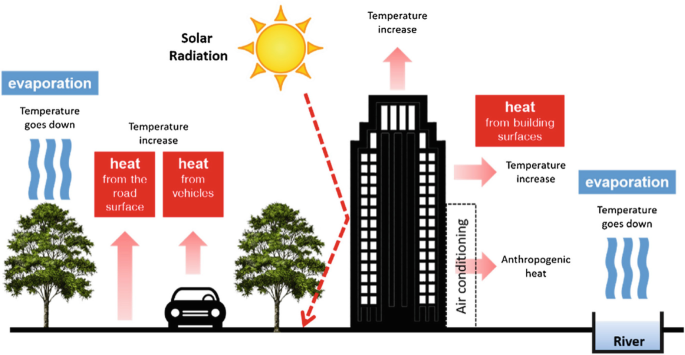
\includegraphics[width=0.7\textwidth]{images/micro-climat_scheme.png} \\
        \end{column}
    \end{columns}

    \vspace{-0.4cm}
    \textbf{Physical models:}
    \begin{itemize}
        \item Continuous physical phenomena: PDEs (Navier-Stokes, heat, transport, diffusion)
        \item Interaction between buildings, wind, vegetation: Fluid-Structure Interaction (NS + Elasticity)
        \item Airflow and heat exchange: Computational Fluid Dynamics (NS + Heat; Transport; radiative transfer) % effet du soleil sur les façades
    \end{itemize}
\end{frame}


\begin{frame}
    \small
    % résolution très lourde et longue à calculer, donc:
    \textbf{ROM usage:} Reducing the order of physical models to speed up simulations  \\
    \vspace{0.2cm}
    - \textbf{Offline:} Model preparation (hours / days)
    \begin{itemize}
        \item Dimension reduction by capturing the essence of the system: Proper Orthogonal Decomposition (POD), Reduced Basis Method (RBM)
        \item Hyper-reduction: Reduces computation time of nonlinear terms (DEIM: Discrete Empirical Interpolation Method, gappy POD: gappy Proper Orthogonal Decomposition) % en évaluant seulement certains points clés du modèle
    \end{itemize}
    \vspace{0.2cm}
    - \textbf{Online:} Simulation of the reduced model to quickly test different scenarios (seconds / minutes)
    \vspace{-0.4cm}
    \begin{flushright}
        \includegraphics[width=0.5\textwidth]{images/diff_scénarios.jpg}
    \end{flushright}
\end{frame}


\begin{frame}
    \small
    \textbf{Data-Driven Models:} data-driven, fast prediction % sur le micro-climat
    \begin{itemize}
        \item Regression: predicts phenomena (temperature, air quality, wind) from variables (materials, vegetation...)
        \item Gaussian Process: predicts and provides uncertainty for areas with little data
    \end{itemize}
    \vspace{-0.3cm}
    \begin{columns}[T]
    \begin{column}{0.6\textwidth}
    \begin{itemize}
        \setlength\itemindent{0.3cm}
        \item Neural Networks: capture complex and non-linear relationships between variables 
        \end{itemize}
    \end{column}

    \begin{column}{0.4\textwidth}
        \vspace{-0.3cm}
        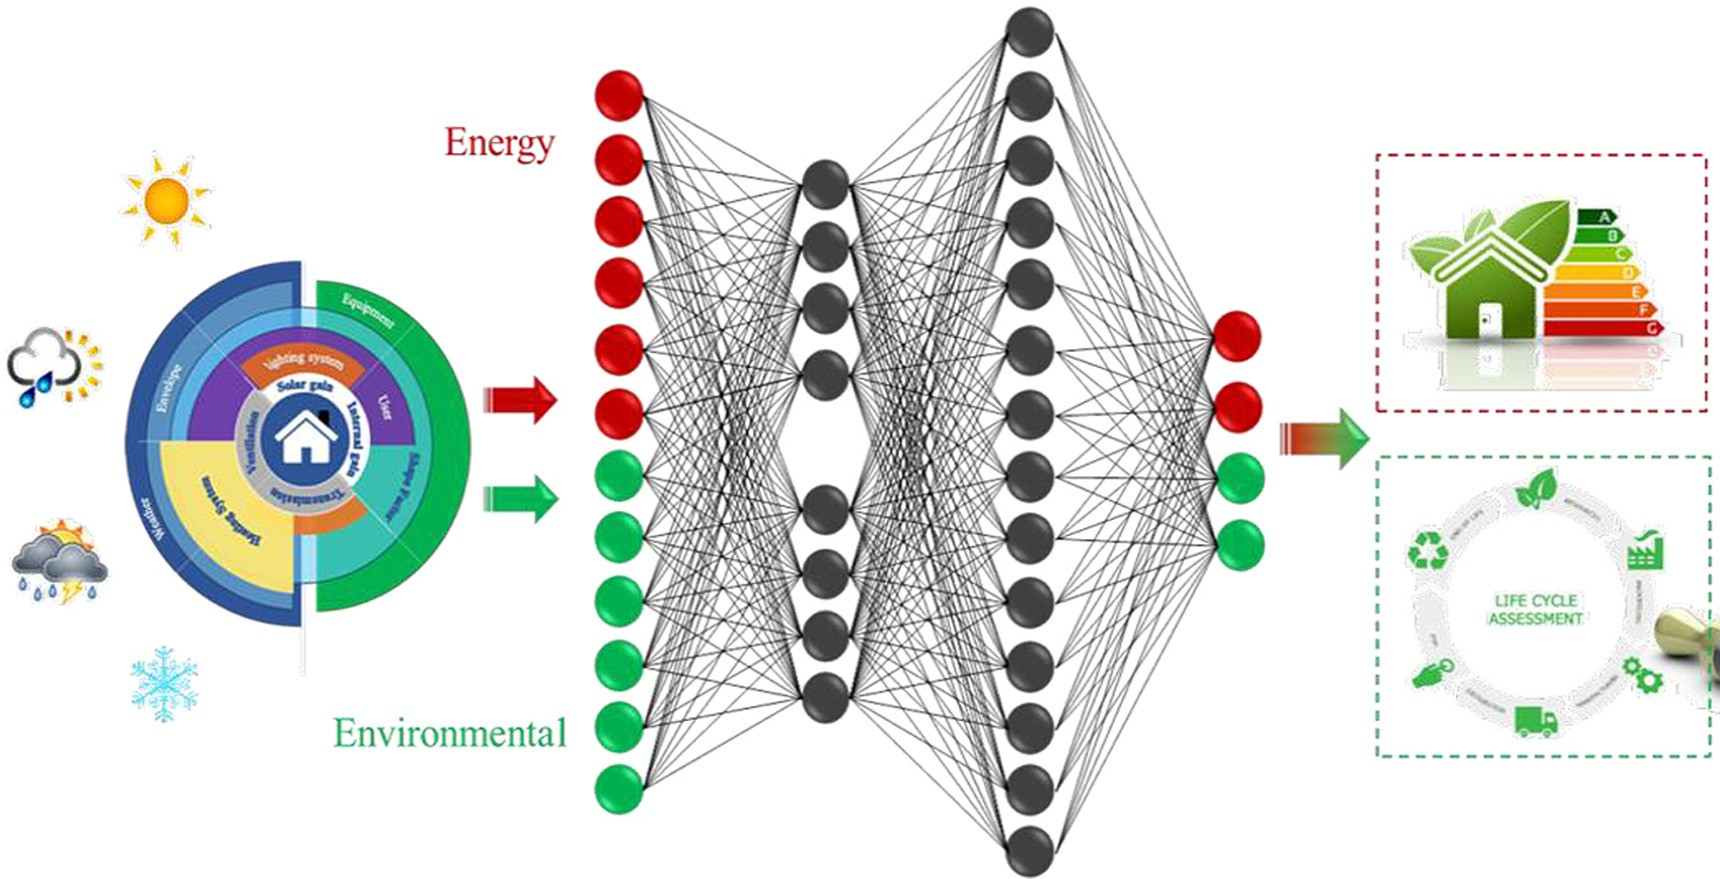
\includegraphics[width=1\textwidth]{images/NN-env.jpg}
    \end{column}
    \end{columns}
    \vspace{-0.3cm}
    \begin{itemize}
        \item Ensemble models: improving prediction \\ accuracy and robustness by combining multiple models
    \end{itemize}
\end{frame}


\begin{frame}
    \small
    \textbf{Data assimilation:} Combining physical models and data to correct simulations, achieve maximum accuracy, and make these simulations usable % pour la prise de décision
    \vspace{0.2cm}
    \begin{itemize}
        \item Vector Auto-Regression (VAR): adjusts the physical model so that simulations match observations (over one or more time steps)
        \item Kalman Filter: Updates predictions in real-time for dynamic tracking
        \item Parameterized-Background Data-Weak (PBDW), Generalized Empirical Interpolation Method (GEIM): reconstructs the system with little data, for an overview
        \item Virtual sensors: estimation of variables where there are no measurements, see the effect of new developments
    \end{itemize}
\end{frame}





\begin{frame}{Data \& Instrumentation — Data Budget (Urban Microclimate)}
\tiny
\setlength{\tabcolsep}{3pt}  
\textit{Goal: quantify sensor data rates and daily volumes to size network \& storage for real-time operation.}

\vspace{2mm}
\begin{tabular}{lcccccc}
\textbf{Sensor} & \textbf{\#} & \textbf{Freq (Hz)} & \textbf{sample} & \textbf{Throughput (kB/s)} & \textbf{Vol/day (GB)} & \textbf{Comments} \\
\hline
Air thermometer (T)   & 20 & 1.00  & 8        & 0.16  & 0.014 & Ambient temperature \\
Hygrometer (RH)       & 10 & 1.00  & 8        & 0.08  & 0.007 & Relative humidity \\
Anemometer (3-axis)   & 5  & 1.00  & 12       & 0.06  & 0.005 & Wind speed \& direction \\
Pyranometer (solar)   & 5  & 0.20  & 16       & 0.016 & 0.0014& Global irradiance \\
Thermal camera*       & 2  & 0.033 & 500{,}000& 33.0  & 2.85  & H.264, store temperature maps \\
\hline
\end{tabular}

\vspace{1mm}
\footnotesize
\textbf{Formulas:}
\begin{block}{Throughput (kB/s) \& Volume/day (GB)}
    $$Throughput (kB/s): \quad = \dfrac{\# \times \text{sample} \times \text{Freq}}{1000}$$
    $$ \noindent Volume/day (GB): \quad = \dfrac{\text{Throughput (kB/s)} \times 86\,400}{10^{6}}$$
\end{block}
\vspace{0.5mm}
\scriptsize
\textbf{Protocols/latency:} LoRaWAN for low-rate sensors (2–5 s latency); Wi-Fi/4G for cameras ($<0.5$ s).  \\
\textbf{Privacy:} camera streams anonymized on edge; only thermal maps stored.
\end{frame}


\begin{frame}{V\&V \& UQ — Verification, Validation \& Uncertainty Quantification}
\centering
\tiny
\begin{block}{Goal}
    \textit{Goal: ensure accuracy, reliability, and safety of decisions in the urban microclimate digital twin.}
\end{block}
\vspace{0.4cm}
\begin{tabular}{|p{2.5cm}|p{3.5cm}|p{4.2cm}|}
\hline
\textbf{Step} & \textbf{Purpose} & \textbf{Methods / Indicators} \\
\hline
\textbf{1️ Verification} &
Check model implementation and numerical stability. &
Compare the Reduced Order Model (ROM) with the full CFD model.  
Ensure no numerical or stability errors. \\
\hline
\textbf{2️ Validation} &
Evaluate how well the model matches real-world data. &
Compare predictions with sensor measurements (T°, wind, humidity).  
Metrics: \textbf{MAE}, \textbf{RMSE}, \textbf{R\textsuperscript{2}}. \\
\hline
\textbf{3️ Uncertainty Quantification (UQ)} &
Estimate the confidence level of model predictions. &
Methods: Monte Carlo, sensitivity analysis, Bayesian estimation.  
Example: $T = 32 \pm 1.5^\circ$C. \\
\hline
\textbf{4️ Veto / Alert Mechanism} &
Prevent wrong or unsafe decisions when uncertainty is too high. &
If confidence interval $>$ threshold → trigger alert or model recalibration. \\
\hline
\end{tabular}

\vspace{0.3cm}
\textit{Outcome: a validated, uncertainty-aware model ensuring trustworthy real-time decisions.}
\end{frame}


\begin{frame}{Transfer \& Deployment — CI/CD, Edge vs Cloud, Observability, Risks}
\centering
\tiny
\begin{block}{Goal}
    \textit{ensure a smooth transition from R\&D to real-time operation of the urban microclimate digital twin.}
\end{block}
\vspace{0.4cm}
\begin{tabular}{|p{2.5cm}|p{3.5cm}|p{4.2cm}|}
\hline
\textbf{Aspect} & \textbf{Description} & \textbf{Tools / Key Points} \\
\hline
\textbf{CI/CD (Continuous Integration \& Deployment)} &
Automate the update cycle for models and data. &
GitHub Actions, Docker, unit tests for ROM/data, dashboard updates. \\
\hline
\textbf{Containers \& Orchestration} &
Ensure portability and scalability of digital twin services. &
Docker / Kubernetes: deployment of ROM model, APIs, dashboards. \\
\hline
\textbf{Edge vs Cloud Computing} &
Balance local computing (edge) and centralized storage (cloud). &
Edge: low latency (cameras, sensors).  
Cloud: heavy computations (assimilation, ROM training). \\
\hline
\textbf{Observability \& Monitoring} &
Track performance, errors, and model drifts. &
Logs, metrics, and alerts through Grafana / Prometheus. \\
\hline
\textbf{Costs \& Risks (CAPEX/OPEX)} &
Optimize hardware resources and minimize downtime. &
CAPEX: servers / sensors.  
OPEX: maintenance, energy, network.  
Risk: failure, model drift. \\
\hline
\end{tabular}

\vspace{0.3cm}
\textit{Outcome: a reliable, automated, and maintainable digital twin for long-term operation.}
\end{frame}


\begin{frame}{Perspectives — Toward a Sustainable Digital Twin}
\small
\begin{itemize}
    \item \textbf{Scalability:} extend the model to larger urban areas using cloud computing and ROM optimization.  
    \item \textbf{Continuous improvement:} integrate new sensors (CO₂, fine particles) and additional data sources (satellite, weather).  
    \item \textbf{Optimization:} further automate calibration and data assimilation for faster model updates.  
\end{itemize}
\vspace{3mm}
\textit{Goal: make the digital twin more complete, faster, and more useful for urban decision-making.}
\end{frame}


\begin{frame}{Limitations and Current Challenges}
\small
\begin{itemize}
    \item \textbf{Robustness:} sensors may fail or produce noisy data so adaptive models are needed.  
    \item \textbf{Bias:} the model can overfit to one district which means multi-scenario validation is required. 
    \item \textbf{Costs:} find the right balance between accuracy, speed, and budget (cloud, maintenance).  
\end{itemize}
\vspace{3mm}
\textit{These challenges highlight what must be improved to make the digital twin reliable and sustainable in the long term.}
\end{frame}


% --- Slide: Acknowledgment / Questions ---
\begin{frame}{Thank You / Questions}
\centering
\Huge \textbf{Thank you for your attention!} \\
\vspace{1cm}
\Large Any questions? \\
\vspace{0.5cm}
\textit{University of Strasbourg – 2025}
\end{frame}



% --- Slide: Références ---
\begin{frame}[allowframebreaks]{Références}
  \nocite{*}
  \bibliographystyle{plain}
  \bibliography{bibliography}
\end{frame}


\end{document}